%
% 1-definition.tex
%
% (c) 2023 Prof Dr Andreas Müller, OST Ostschweizer Fachhochschule
%
\section{Definition
\label{buch:radon:section:definition}}
\kopfrechts{Definition}
Die Radon-Transformation zerlegt die Fourier-Transformation in 
mehr als einer Dimension in Integrale parallel und senkrecht
zur ``Richtung'' einer Welle.
In diesem Abschnitt wird die Radon-Transformation zunächst aus der
zweidimensionalen Fourier-Transformation motiviert und anschliessend
für Funktionen in beliebiger Dimension definiert.

%
% Zweidimensionale Fourier-Transformation
%
\subsection{Zweidimensionale Fourier-Transformation
\label{buch:radon:definition:subsection:2dfourier}}
Für die zweidimensionale Fourier-Transformation muss zunächst die
duale Gruppe der additiven Gruppe $\mathbb{R}^2$ ermittelt werden,
dann folgend die Formeln für die Fourier-Transformation und die
Rücktransformation fast automatisch.

%
% Die duale Gruppe von R^2
%
\subsubsection{Die duale Gruppe von $\mathbb{R}^2$}
Die duale Gruppe von $\mathbb{R}^2$ besteht aus den stetigen
Homomorphismen von der additiven Gruppe $\mathbb{R}^2$ in die
multiplikative Gruppe $\mathbb{C}^*$.
Ein Homomorphismus ist eine Funktion
\[
\varphi
\colon
\mathbb{R}^2\to\mathbb{C}^*
:
(x,y)\mapsto \varphi(x,y)
\]
mit der Eigenschaft
\begin{equation}
\varphi(x+x',y+y')
=
\varphi(x,y)
\varphi(x',y').
\label{buch:radon:definition:eqn:homomorphismus}
\end{equation}
Setzt man eine der Variablen $=0$ entsteht die eindimensionale Situation,
% XXX wo?
die früher bereits untersucht wurde.
Die Funktionen
\begin{equation*}
\begin{aligned}
\varphi(\cdot,0)&\colon \mathbb{R} \to \mathbb{C}^*&:
x\mapsto &\varphi(x,0)
\\
\varphi(0,\cdot)&\colon \mathbb{R} \to \mathbb{C}^*&:
y\mapsto &\varphi(0,y)
\end{aligned}
\end{equation*}
sind stetige Homomorphismen und daher Exponentialfunktionen der Form
\[
\varphi(x,0) = e^{ikx}
\qquad\text{und}\qquad
\varphi(0,y) = e^{ily}
\]
mit $k,l\in\mathbb{R}$.
Aus der
Homomorphismuseigenschaft~\eqref{buch:radon:definition:eqn:homomorphismus}
folgt dann
\[
\varphi(x,y)
=
\varphi(x,0)\varphi(0,y)
=
e^{ikx}e^{ily}
=
e^{i(kx+ly)}.
\]
Wir schreiben $\varphi_{kl}(x,y) = e^{i(kx+ly)}$ wenn es nötig ist, die
Parameter $k$ und $l$ explizit zu machen.
Die Menge der Homomorphismen $\operatorname{Hom}(\mathbb{R}^2,\mathbb{C}^*)$
ist daher parametrisiert durch die Paare $(k,l)\in\mathbb{R}^2$.

Die Gruppenoperation der Homomorphismen verträgt sich mit der additiven
Struktur von $\mathbb{R}^2$.
Das Produkt zweier Homomorphismen mit Parameter $k_1,l_1$ bzw.~$k_2,l_2$
ist
\[
\varphi_{k_1,l_1}(x,y)
\varphi_{k_2,l_2}(x,y)
=
e^{i(k_1x+l_1y)}
e^{i(k_2x+l_2y)}
=
e^{i((k_1+k_2)x+(l_1+l_2)y)}
=
\varphi_{k_1+k_2,l_1+l_2}(x,y).
\]
Die Abbildung $(k,l)\mapsto \varphi_{kl}$ ist daher ein Isomorphismus
der Gruppe $\mathbb{R}^2$ auf die duale Gruppe von $\mathbb{R}^2$,
es ist $\widehat{\mathbb{R}^2} = \mathbb{R}^2$.

%
% Ebene Wellen
%
\subsubsection{Ebene Wellen}
\begin{figure}
\centering
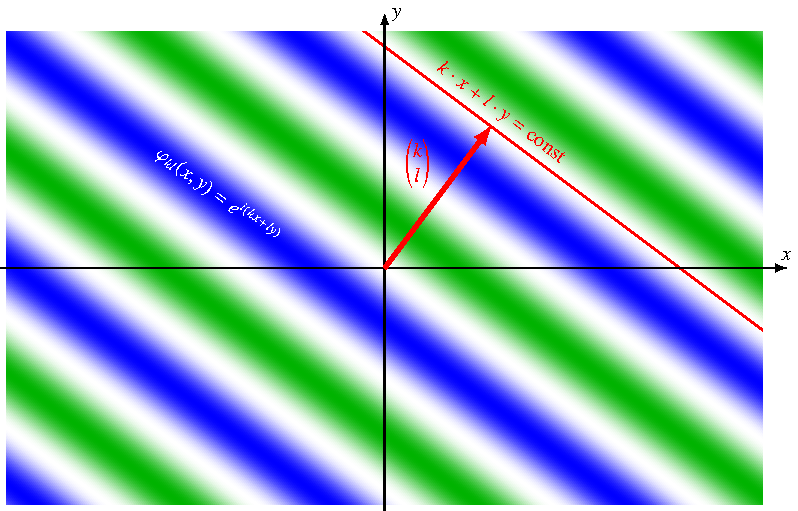
\includegraphics{chapters/050-radon/images/ebenewellen.pdf}
\caption{Ebene Welle $\varphi_{kl}(x,y)$ mit Ausbreitungsrichtung
in Richtung des Wellenvektors mit den Komponenten $k$ und $l$.
Die Wellenfronten stehen senkrecht auf dem Wellenvektor.
\label{buch:radon:fig:ebenewelle}}
\end{figure}
Wie Abbildung~\ref{buch:radon:fig:ebenewelle} zeigt, sind
die Funktionen $\varphi_{kl}(x,y)$ beschreiben ebene Wellen.
Die Abbildung zeigt nur die Werte des Imaginärteils $\Im \varphi_{kl}(x,y)$,
blau für negative Werte und grün für negative Werte.
$\varphi_{kl}(x,y)$ ist konstant auf der Menge der Punkte, für die
$kx+ly$ konstant ist.
Da dies das Skalarprodukt 
\[
kx+ly 
=
\begin{pmatrix}x\\y\end{pmatrix}
\cdot
\begin{pmatrix}k\\l\end{pmatrix}
\]
ist, ist $\varphi_{kl}(x,y)$ konstant auf Geraden mit der Normalen
mit Komponenten $k$ und $l$, dem sogenannten Wellenvektor.

%
% Die duale Gruppe von $(R/2\pi Z)^2$
%
\subsubsection{Die duale Gruppe von $(\mathbb{R}/2\pi\mathbb{Z})^2$}
Homomorphismen von der additiven Gruppe $(\mathbb{R}/2\pi\mathbb{Z})^2$
nach $\mathbb{C}^*$ sind Homomorphismen $\mathbb{R}^2\to\mathbb{C}^*$,
sie lassen sich also auf jeden Fall als Exponentialfunktionen schreiben.
Ausserdem müssen Sie aber in jedem Argument $2\pi$-periodisch sein.
Die Funktion $\varphi_{kl}$ ist genau dann im ersten Argument
$2\pi$-periodisch, wenn die partielle Funktion
$x\mapsto \varphi_{kl}(x,0) = e^{ikx}$ schon $2\pi$-periodisch ist,
was nur möglich ist, wenn $k\in\mathbb{Z}$.
Auf die gleiche Weise folgt auch, dass $l\in\mathbb{Z}$ sein muss.
Die duale Gruppe von $(\mathbb{R}/2\pi\mathbb{Z})^2$ ist daher
die Gruppe $\mathbb{Z}^2$ der ganzzahligen Wellenvektoren.

%
% Fourier-Transformation
%
\subsection{Fourier-Transformation}
Nach der Gelfand-Theorie ordnet die Transformation, die aus der Faltung
ein Produkt macht, der Funktion $f(x,y)$ die Funktion
\begin{equation}
(\mathscr{F}f)(k,l)
=
\frac{1}{2\pi} \int_{\mathbb{R}^2} \overline{\varphi}_{kl}(x,y)\,f(x,y)\,dx\,dy
=
\frac{1}{2\pi} \int_{\mathbb{R}^2} e^{-i(kx+ly)}\,f(x,y)\,dx\,dy
\label{buch:radon:eqn:2dfourier:def}
\end{equation}
zu.
Das Doppelintegral
\eqref{buch:radon:eqn:2dfourier:def}
kann wegen der Faktorisierung $\varphi_{kl}(x,y)=e^{ikx}\cdot e^{ily}$
in zwei Integrale der Form
\begin{align}
(\mathscr{F}f)(k,l)
&=
\frac{1}{\!\sqrt{2\pi}}\int_{-\infty}^\infty
e^{-ikx}
\frac{1}{\!\sqrt{2\pi}}\int_{-\infty}^\infty
e^{-ily}
f(x,y)
\,dy
\,dx
\label{buch:radon:2dfourier:eqn:f2f1}
\intertext{oder}
&=
\frac{1}{\!\sqrt{2\pi}}\int_{-\infty}^\infty
e^{-ily}
\frac{1}{\!\sqrt{2\pi}}\int_{-\infty}^\infty
e^{-ikx}
f(x,y)
\,dx
\,dy
\label{buch:radon:2dfourier:eqn:f1f2}
\end{align}
aufgeteilt werden.
Die inneren Integrale sind dabei einfache Fourier-Transformationen
der partiellen Funktionen $y\mapsto f(x,y)$ bzw.~$x\mapsto f(x,y)$
mit einem freien Parameter $x$ bzw.~$y$.
Die Wahl des Normierungsfaktors ist somit konsistent mit dem bei der
eindimensionalen Transformation verwendeten.
Schreibt man $\mathscr{F}_x$ und $\mathscr{F}_y$ für die eindimensionale
Fourier-Transformation der Variablen $x$ bzw.~$y$, dann kann man
die Ingegrale \eqref{buch:radon:2dfourier:eqn:f2f1}
und \eqref{buch:radon:2dfourier:eqn:f1f2}
auch als die Zusammensetzungen der Transformationen
\[
\mathscr{F}
=
\mathscr{F}_x\mathscr{F}_y
=
\mathscr{F}_y\mathscr{F}_x
\]
lesen.

Auch die Umkehrtransformation kann man sofort ablesen, sie muss
\begin{align*}
\mathscr{F}^{-1}g (x)
&=
\frac{1}{2\pi}\int_{\mathbb{R}^2}
e^{i(kx+ly)}g(k,l)
\,dk\,dl
\intertext{mit den Faktorisierungen}
&=
\frac{1}{\!\sqrt{2\pi}}\int_{-\infty}^\infty
e^{ikx}
\frac{1}{\!\sqrt{2\pi}}\int_{-\infty}^\infty
e^{ily}
g(k,l)
\,dl\,dk
\intertext{und}
&=
\frac{1}{\!\sqrt{2\pi}}\int_{-\infty}^\infty
e^{ily}
\frac{1}{\!\sqrt{2\pi}}\int_{-\infty}^\infty
e^{ikx}
g(k,l)
\,dk\,dl
\end{align*}
sein.
Die einfachen Integrale sind wieder Fourier-Umkehrtransformationen
für die partiellen Funktionen von $g$.
Es gilt also auch
\[
\mathscr{F}^{-1}
=
\mathscr{F}_x^{-1} \mathscr{F}_y^{-1}
=
\mathscr{F}_y^{-1} \mathscr{F}_x^{-1}.
\]

%
% Integrale über Hyperebenen
%
\subsection{Integrale über Geraden
\label{buch:radon:definition:subsection:geraden}}
\begin{figure}
\centering
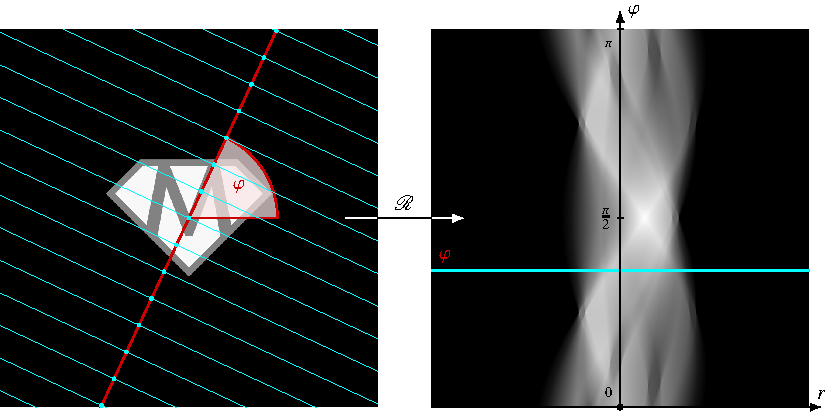
\includegraphics[width=\textwidth]{chapters/050-radon/images/radon.pdf}
\caption{Die Radon-Transformation berechnet Integrale über Geraden
senkrecht auf die Richtung mit Polarwinkel $\varphi$.
\label{buch:radon:definition:fig:radon}}
\end{figure}
Wir betrachten jetzt eine Funktion $u\colon \mathbb{R}^2\to\mathbb{C}$,
deren Fourier-Transformierte berechnet werden soll.
Die Fourier-Transformierte von $u$ ist die Funktion
\[
\mathscr{F}u(k,l)
=
\frac{1}{2\pi}
\int_{\mathbb{R}^2}
\overline{\varphi}_{kl}(x,y)
u(x,y)
\,dx\,dy
=
\frac{1}{2\pi}
\int_{\mathbb{R}^2}
e^{-i(kx+ly)}
u(x,y)
\,dx\,dy.
\]
Der Exponent $kx+ly$ ist konstant entlang von Geraden, die
senkrecht auf dem Vektor mit den Komponenten $(k,l)$ stehen
(Abbildung~\ref{buch:radon:fig:ebenewellen}).
Entlang solcher Geraden ist daher auch $e^{i(kx+ly)}$ konstant.
Wählt man ein Koordinatensystem so, dass diese Geraden
Koordinatenachsen werden, kann das Fourier-Integral zerlegt werden.

Durch Drehung um den Winkel $\alpha$ mit der Drehmatrix
\[
D_\alpha
=
\begin{pmatrix*}
\cos\alpha&-\sin\alpha\\
\sin\alpha& \cos\alpha
\end{pmatrix*}
\]
erzeugt den Vektor mit den Komponenten $k$ und $l$ aus einem
Vektor, der parallel zur $x$-Achse verläuft.
Es ist nämlich
\[
\begin{pmatrix}k\\l\end{pmatrix}
=
D_\alpha
\begin{pmatrix}\kappa\\0\end{pmatrix}
=
\begin{pmatrix}
\kappa\cos\alpha\\
\kappa\sin\alpha
\end{pmatrix},
\]
wenn man $\alpha$ als Winkel zwischen der $x$-Achse und Richung
des Vektors mit den Komponenten $k$ und $l$ wählt und
$\kappa=\!\sqrt{k^2+l^2}$ setzt.

Die Koordinatentransformation
\[
\begin{pmatrix}
x\\
y
\end{pmatrix}
=
D_\alpha
\begin{pmatrix}
\xi\\
\eta
\end{pmatrix}
\]
ist eine Isometrie, wegen $\det D_\alpha=1$ ändert sie das Integral
nicht, es folgt also
\begin{equation}
\mathscr{F}u(k,l)
=
\frac{1}{2\pi}
\int_{-\infty}^\infty
e^{-i\kappa \xi} \tilde{f}(\xi,\eta)\,d\xi\,d\eta,
\label{buch:radon:definition:eqn:fgedreht}
\end{equation}
wobei wir
\[
\tilde{f}(\xi,\eta)
=
f(\xi\cos\alpha-\eta\sin\alpha,\xi\sin\alpha+\eta\cos\alpha)
\]
abkürzen.
Das Doppelintegral~\eqref{buch:radon:definition:eqn:fgedreht}
kann in in zwei einfache Integrale
\begin{align*}
\mathscr{F}u(k,l)
&=
\frac{1}{\!\sqrt{2\pi}}
\int_{-\infty}^\infty
e^{-i\kappa\xi}
\frac{1}{\!\sqrt{2\pi}}
\int_{-\infty}^\infty
\tilde{f}(\xi,\eta)
\,d\eta
\,d\xi.
\intertext{%
Das innere Integral ist ein Integral der Funktion $\tilde{f}$
über die Gerade $\xi=\operatorname{const}$.
Das äussere Integral ist eine gewöhnliche eindimensionale
Fourier-Transformation der Variablen $\xi$.
}
&=
\frac{1}{\!\sqrt{2\pi}}
\int_{-\infty}^\infty
e^{-i\kappa\xi}
\frac{1}{\!\sqrt{2\pi}}
\int_{-\infty}^\infty
f(\xi\cos\alpha-\eta\sin\alpha,\xi\sin\alpha+\eta\cos\alpha)
\,d\eta
\,d\xi.
\end{align*}
Das innere Integral ist über die Gerade mit der Parameterdarstellung
\[
\eta
\begin{pmatrix}
\cos\alpha\\
\sin\alpha
\end{pmatrix}
+
\eta
\begin{pmatrix}
-\sin\alpha\\
\cos\alpha
\end{pmatrix}.
\]
Sie ist die Gerade orthogonal zum Vektor
\[
\omega
=
\begin{pmatrix}
-\sin\alpha\\
\cos\alpha
\end{pmatrix}
\]
im Abstand $\xi$ vom Ursprung des Koordinatensystem.

%
% Die Radon-Transformation
%
\subsection{Die Radon-Transformation
\label{buch:radon:definition:subsection:radon}}
Die Zerlegung der Fourier-Transformation in der Ebene in ein Integral
über Geraden senkrecht auf $\omega$ und eine Fourier-Transformation 
in Richtung von $\omega$.
Diese Idee lässt sich jetzt aber auf beliebige Dimension verallgemeinern.

%
% Die n-1-dimensionalen Sphären
%
\subsubsection{Die $n-1$-dimensionalen Sphären}
Die Geraden in der Ebene waren beschrieben durch den Richtungsvektor
$\omega$ und den Abstand der Geraden vom Ursprung.
Der Richtungsvektor ist ein Einheitsvektor.
In $\mathbb{R}^n$ müssen also die Einheitsvektoren zur Parametrisierung
verwendet werden.

\begin{definition}
Die $n-1$-dimensionale Sphäre ist die Teilmenge
\[
S^{n-1}
=
\{
x\in\mathbb{R}^n
\mid
|x|=1
\}.
\]
\end{definition}

In der Ebene, also für $n=2$ lassen sich die Vektoren $\omega\in S^1$
mit trigonometrischen Funktionen parametrisieren.
Solche Parametrisierungen sind auch möglich für $n>2$, in drei
Dimensionane zum Beispiel könnten Kugelkoordinaten verwendet werden.
Allerdings benötigen wir im folgenden gar keine explizite Parametrisierung
und verzichten daher darauf, eine solche anzugeben.

%
% Hyperebenen
%
\subsubsection{Hyperebenen}
Die Hyperebenen, über die integriert werden soll, werden durch die
Richtung $\omega\in S^{n-1}$ und den Abstand vom Nullpunkt des
Koordinatensystems parametrisiert.

\begin{definition}
Für $s\in\mathbb{R}$ und $\omega\in S^{n-1}$ bezeichnen wir mit
\[
E(s,\omega)
=
\{
x\in\mathbb{R}^n
\mid
\omega\cdot x = s
\}
\subset
\mathbb{R}^n
\]
die Hyperebene orthogonal auf $\omega$ im Abstand $s$ vom Ursprung.
\end{definition}

Durch Wahl eines geeigneten Koordinatensystems kann man ein
Integral über $\mathbb{R}^n$ immer schreiben als
ein Integral über die Ebenen $E(s,\omega)$ und eines über die Koordinaten $s$.
Ein solches Koordinatensystem kann zum Beispiel gefunden werden, indem
man den Vektor $\omega\in S^{n-1}$ mit Vektoren $b_2,\dots,b_n$ zu einer
Orthonormalbasis von $\mathbb{R}^n$ erweitert.
Das Integral über $\mathbb{R}^n$ ist dann
\[
\int_{\mathbb{R}^n} f(x)\,dx
=
\int_{-\infty}^\infty
\int_{\mathbb{R}^{n-1}}
f(s\omega + \xi_2 b_2+\dots \xi_n b_n)
\,d\xi_2\dots\,d\xi_n
\,ds.
\]
Die Wahl der Basisvektoren $b_2,\dots,b_n$ hat keinen Einfluss
auf den Wert des Integrals.
Mit der Abkürzung
\[
\xi
=
\sum_{k=2}^n
\xi_k b_k
\]
ist es daher zulässig, das Integral einfach als
\[
\int_{\mathbb{R}^n} f(x)\,dx
=
\int_{-\infty}^\infty
\int_{\mathbb{R}^{n-1}}
f(s\omega + \xi)
\,d\xi
\,ds
\]
zu schreiben.
Die Vektoren $s\omega +\xi$ sind die Punkte der Ebene $E(s,\omega)$,
wir können daher das Integral noch einfacher als
\[
\int_{\mathbb{R}^n} f(x)\,dx
=
\int_{-\infty}^\infty
\int_{E(s,\omega)}
f(\xi)
\,d\mu(\xi)
\,ds
\]
schreiben, wobei wir mit $d\mu$ das Volumenelement der Hyperebene
$E(s,\omega)$ meinen.

%
% Radon-Transformation
%
\subsubsection{Radon-Transformation}
Die Fourier-Transformation einer Funktion $u\colon \mathbb{R}^n\to\mathbb{C}$
ist das $n$-fache Integral
\[
\mathscr{F}u(k)
=
\frac{1}{(2\pi)^{\frac{n}2}}
\int_{\mathbb{R}^n}
e^{-ik\cdot x} u(x)\,dx.
\]
Der Exponent der Exponentialfunktion ist konstant auf Hyperebenen senkrecht
auf dem Vektor $k$.
Schreiben wir $k=k_0k^0=k_0\omega$ mit $\omega=k^0$, wobei $k^0=k/|k|$ der
zu $k$ gehörige Einheitsvektor ist, dann ist 
$E(k_0,k^0)$ die Hyperebene, auf der der Exponentialfaktor den
Wert $e^{-ik_0\omega\cdot x}$ hat.
Die Fourier-Transformation wird dann
\[
\mathscr{F}u(k_0\omega)
=
\frac{1}{(2\pi)^{\frac{n}2}}
\int_{\mathbb{R}}
e^{-ik_0r}
\int_{E(k_0,\omega)}
u(\xi)
\,d\mu(\xi)
\,dr.
\]
Das innere Integral ist die gesuchte Transformation:

\begin{definition}
Sei $u\colon\mathbb{R}^n\to\mathbb{C}$ eine integrierbare Funktion,
dann heisst die Funktion
\[
\mathscr{R}u
\colon
\mathbb{R}\times S^{n-1}
\to
\mathbb{C}
:
(s,\omega)
\mapsto
\mathscr{R}(r,\omega)
=
\int_{E(r,\omega)} u(\xi) \,d\mu(\xi)
\]
die {\em Radon-Transformierte} von $u$.
\index{Radon-Transformierte}%
Die Transformation $u\mapsto \mathscr{R}u$ heisst die
{\em Radon-Transformation}.
\index{Radon-Transformation}%
\end{definition}

%
% Radon- und Fourier-Transformation
%
\subsection{Radon- und Fourier-Transformation
\label{buch:radon:definition:subsection:radonfourier}}
\begin{figure}
\centering
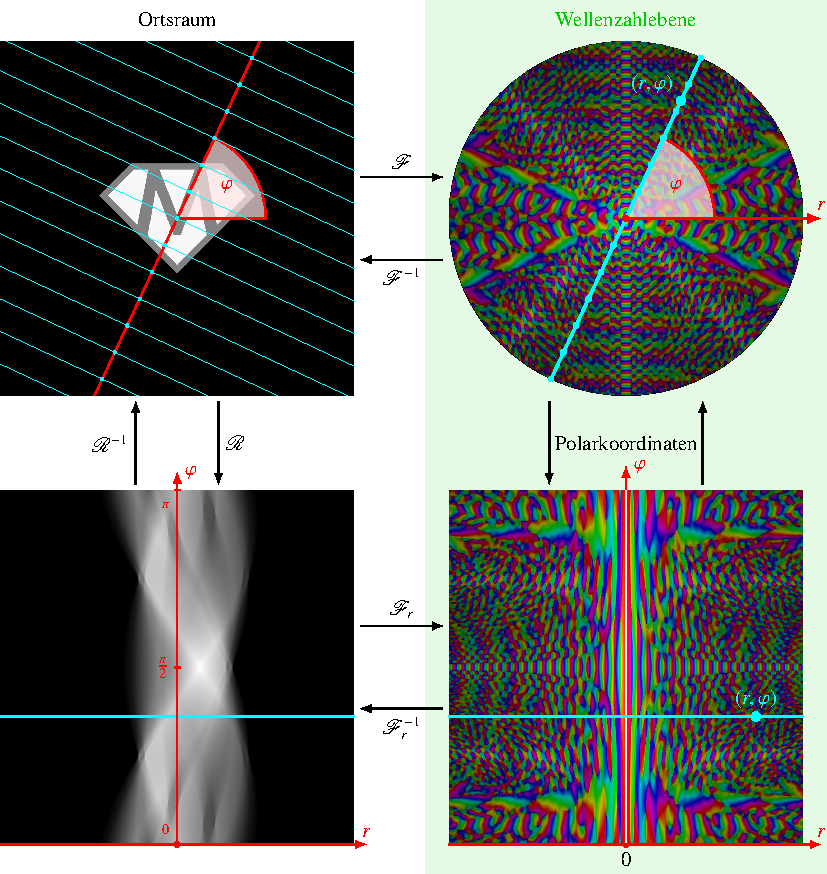
\includegraphics[width=\textwidth]{chapters/050-radon/images/radonft.pdf}
\caption{Zusammenspiel der Radon- und Fourier-Transformation.
Die Radontransformation $\mathscr{R}$ gefolgt von einer (radialen)
Fourier-Transformation $\mathscr{F}_r$, die nur die $r$-Koordinate
betrifft, wird zur einer Fourier-Transformation $\mathscr{F}$, wenn
man die $(r,\varphi)$ als Polarkoordinaten der Wellenzahl-Ebene
(rechte Hälfte der Abbildung) interpretiert.
\label{buch:radon:definition:fig:radonft}}
\end{figure}
Die Radon-Transformation vollzieht also einen Teil der Integrationen,
die für das Fourier-Integral erforderlich sind.
Es verbleibt aber immer noch eine Integration, die noch
durchgeführt werden muss, um die Fourier-Transformierte
\[
\mathscr{F}u(k)
=
\mathscr{F}u(k_0\omega)
=
\frac{1}{(2\pi)^{\frac{n-1}2}}
\frac{1}{\!\sqrt{2\pi}}
\int_{\mathbb{R}}
e^{-ik_0r}
\mathscr{R}u(r,\omega)\,dr
\]
zu finden.
Das Integral ist eine gewöhnliche eindimensionale Fourier-Transformation
für die Variable $r$.
Mit der früheren Notation für eindimensionale Fourier-Transformationen
können wir dies schreiben als
\begin{equation}
\mathscr{F}u(k)
=
\frac{1}{(2\pi)^{\frac{n-1}2}}
(\mathscr{F}_r \mathscr{R}u(r,k^0))(|k|).
\label{buch:radon:definitionb:eqn:fr}
\end{equation}
Die Fourier-Transformierte von $u$ kann also gefunden werden,
indem erst die Radon-Transformierte bestimmt wird und anschliessend
bezüglich der ersten Variablen Fourier-transformiert wird.

Die Zusammenetzung~\eqref{buch:radon:definitionb:eqn:fr}
der Fourier-Transformation $\mathscr{F}$ aus
einer eindimensionalen, radialen Transformation $\mathscr{F}_r$ und der
Radon-Transformation $\mathscr{R}$
hat als unmittelbare Konsequenz, dass die Radon-Transformation
invertierbar sein muss.
Ist $v=\mathscr{R}u$, dann kann $u$ zurückgewonnen werden, indem
erst mit einer eindimensionalen Fourier-Transformation die
Fourier-Transformierte $\mathscr{F}u$ bestimmt wird.
Die Funktion $u$ wird dann als Fourier-Umkehrtransformierte davon
gefunden.

\begin{satz}
Ist $u\colon \mathbb{R}^n \to\mathbb{C}$ eine integrierbare Funktion
und $\mathscr{R}u$ ihre Radon-Transformierte, dann ist die
Fourier-Transformierte
\begin{equation}
(\mathscr{F}u)(k)
=
(\mathscr{F}_r \mathscr{R}u)(k^0, r))(|k|)
\label{buch:radon:definition:satzeqn:fourier}
\end{equation}
von $u$ die Zusammensetzung der Radon-Transformation mit der 
eindimensionalen radialen Fourier-Transformation.
\end{satz}

Da die Fourier-Transformation invertierbar ist, können wir schliessen,
dass auch die Radon-Transformation invertierbar ist.
Aus der Gleichung
\eqref{buch:radon:definition:satzeqn:fourier}
kann man ableiten, dass man $u$ aus $\mathscr{R}u$ bekommen kann,
indem man zuerst die Radon-Transformierte bezüglich der Variablen
$r$ Fourier-Transformiert und anschliessend die entstandene 
Funktion von $k$ $n$-dimensional Fourier-rücktransformiert.

\begin{satz}
Ist $u\colon \mathbb{R}^n\to\mathbb{C}$ eine integrierbare Funktion
und $\mathscr{R}u$ ihre Radon-Transformierte, dann kann die Funktion
mit der Umkehrformel
\begin{equation}
u(x)
=
\frac{1}{(2\pi)^n}
\int_{\mathbb{R}^n}
e^{ik\cdot x}
\int_{\mathbb{R}}
e^{-i|k|s}
\mathscr{R}u(s,k^0)
\,ds
\,dk
\label{buch:radon:definition:eqn:radonumkehr}
\end{equation}
bestimmt werden.
\end{satz}

\begin{proof}[Beweis]
Das innere Integral von \eqref{buch:radon:definition:eqn:radonumkehr}
ist die radiale Fourier-Transformation, das äussere ist die
Fourier-Umkehrformel.
\end{proof}

Der Nachteil ist allerdings, dass diese Vorgehensweise zur Umkehr der
Radon-Transformation nicht unbedingt besonders stabil ist.
In nachfolgenden Abschnitten sind daher bessere Verfahren gesucht,
wie die Radon-Transformation invertiert werden kann.

%
% Anwendungen der Radon-Transformation
%
\subsection{Anwendungen der Radon-Transformation
\label{buch:radon:definition:subsection:anwendungen}}
Die Radon-Transformation hat interessante Anwendungen in Bildgebenden
Verfahren der Medizin.
Ein Computertomograph oder CAT-Scanner bestimmt die Absorbtion von
Röntgenstrahlen, die in einer Ebene den Körper durchdringen.
Dies ist die Radontransformation der Funktion des Absorbtionskoeffizienten
in der Schnittebene.
Durch Invertierung der Transformation kann ein Schnittbild durch
den Körper gewonnen werden.
Die Details dieses Verfahrens werden in Kapitel~\ref{chapter:ct}
ausgeführt.

Ein Magnetresonanzimager (MRI) verwendet Kernspinresonanz in einem Magnetfeld,
um das Integral über die Dichte gewisser Atomkerne über eine Ebene durch
den Körper zu bestimmen.
Er bestimmt also die Radon-Transformation einer Funktion auf $\mathbb{R}$.
Durch Invertierung der Transformation kann die Funktion rekonstruiert werden
und es können Schnittbilder oder dreidimensionale Visualisierungen
der inneren Organe berechnet werden.


